\chapter{Evaluation}\label{chap:evaluation}
To evaluate the effectiveness of our models we evaluate them in offline and online settings. The details of these can be found in Section~\ref{sec:offeval} and \ref{sec:oneval} respectively. Before that, we will discuss the peculiarities of evaluating approaches to citation recommendation in Section~\ref{sec:citrecspecial}.

\section{Special considerations for citation recommendation}\label{sec:citrecspecial}
The goal in many recommendation domains is to identify items a user is likely to engage with, like finding products a user might buy or media a user might want to consume. The relevance judgement of a recommended item in such a case is merely based on the user's subjective taste.
% In other words, if the reciever of a recommendation is satisfied with it, there is no ground for arguing that the recommendation was wrong.
With citations there is more to it than just preference. For a recommended citation to be useful to a researcher it has to be appropriate. To give an example, if the video platform PeerTube recommends a user to watch \emph{Paywall: The Business of Scholarship} there is no scenario in which this could be considered wrong. However, if a citation recommendation system suggests to cite \emph{Alan Turing, ``On Computable Numbers, with an Application to the Entscheidungsproblem'', 1937} in the context \emph{``We use CiteSeerX [] for our evaluation.''}, then this is arguably not usable. This circumstance makes the evaluation of approaches to citation recommendation comparably difficult, because the accurate judgement of relevance (and by extension applicability) of a recommended item for a given input requires expert knowledge. This has to be kept in mind when automatically generating ground truths for offline evaluations and also when interpreting evaluation results.

% Their purpose is not to please their author, but to relate new scholarly work to existing one by means of attribution, backing, critique etc. As a tool in the rather rigid realm of scientific discourse, they have to abide by established conventions and reflect reality. While a movie recommendation cannot be wrong, a citation recommendation easily can.

A common method for evaluating recommender systems is to use items that have existing relevance judgements (e.g. movies with user ratings logged on a website) as an input to the system and compare the output with the actual user judgement. A similar practice exists in citation recommendation. Citation contexts from existing publications are stripped of their citations, fed into the recommender and the result is compared to the original citation. 

depending on citation type more than one citation can be relevant, re-prediction test only for one

blindly taking published author's judgement as ground truth (could be poorly chosen/misinformed; *is* certainly biased)

also a cited doc's role (how it is cited) can develop over time\cite{Swales1986,He2018}


train/test splitting (per cited doc, temporal, ...), re-recommendation, number of contexts describing a recommendation item, ...

% candidates are only citations within current paper\cite{Duma2014}

\section{Offline evaluation}\label{sec:offeval}

how baseline was chosen (TFIDF performed better than BM25 probably b/c length difference of single context vs. aggregated contexts of a cited doc)

FoS doesn't really work, can bring miiinimal plus to bow

count adjacent cits for arXiv, info not available for other data sets

% pre-filtering experiments (knn\cite{Bhagavatula2018}, lsi, lda, fos, ...)
% different evaluation settings (all, CSonly, comparison to MAG, ACL (data from \cite{Faerber2018b})...)
% FoS alone, restrictively combined w/ BOW, only directly preceeding, ...
% PP model alone, combined, ...

% -> not \emph{generally} applicable/beneficial but for certain citation types ...

% also mention \cite{Kobayashi2018} here b/c they specifically target cases where more than one citation is applicable (could be interpreted as either \emph{multiple (simultaneously)} for one context or \emph{several options that are all valid by themselves but in the end a single one is to be chosen} for one contexts)

\begin{table}[]
\centering
    \caption{Key properties of data sets used for evaluation.}
    \label{tab:datasetprops}
\begin{center}
    \begin{tabular}{llrrrr}
    \toprule % CC/RC = citation contexts per recommendation candidate
    Data set & Train/test split & \#Cand. & \#Tested & \#Test set items & Mean CC/RC (SD)\\ 
    \midrule
    arXiv & $\le$2016 / $\ge$2017 & 63,239 & 49,980 & 490,018 & 21.7 (\hphantom{1}51.2) \\
    MAG & $\le$2017 / $\ge$2018 & 45,580 & 8,013 & 53,151 & 69.2 (137.3) \\
    RefSeer & $\le$2011 / $\ge$2012 & 184,539 & 17,323 & 53,401 & 18.2 (\hphantom{1}47.0)\\
    ACL-ARC & $\le$2005 / $=$2006 & 2,431 & 1,089 & 3,881 & \hphantom{1}6.8 (\hphantom{10}9.5) \\
    \bottomrule
    \end{tabular}
\end{center}
\end{table}

\begin{figure}
  \centering
    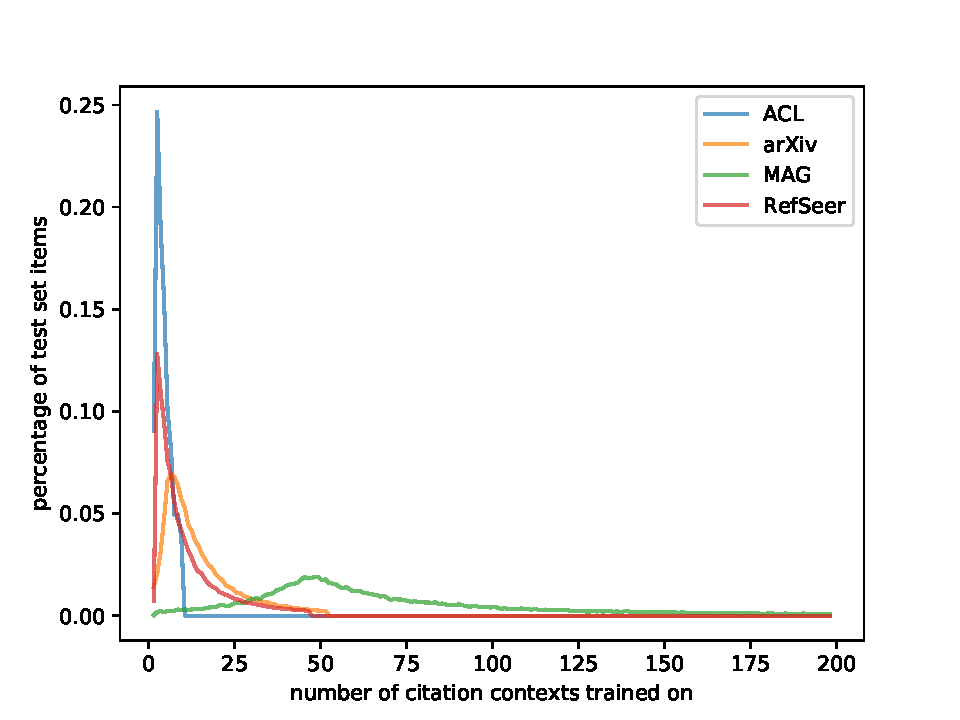
\includegraphics[width=.8\textwidth]{figures/evaluation/comparison_contexts_per_cited_doc.pdf}
  \label{fig:evalcomp}
  \caption{Number of citation contexts per recommendation candidate.}
\end{figure}

\begin{figure}
  \centering
    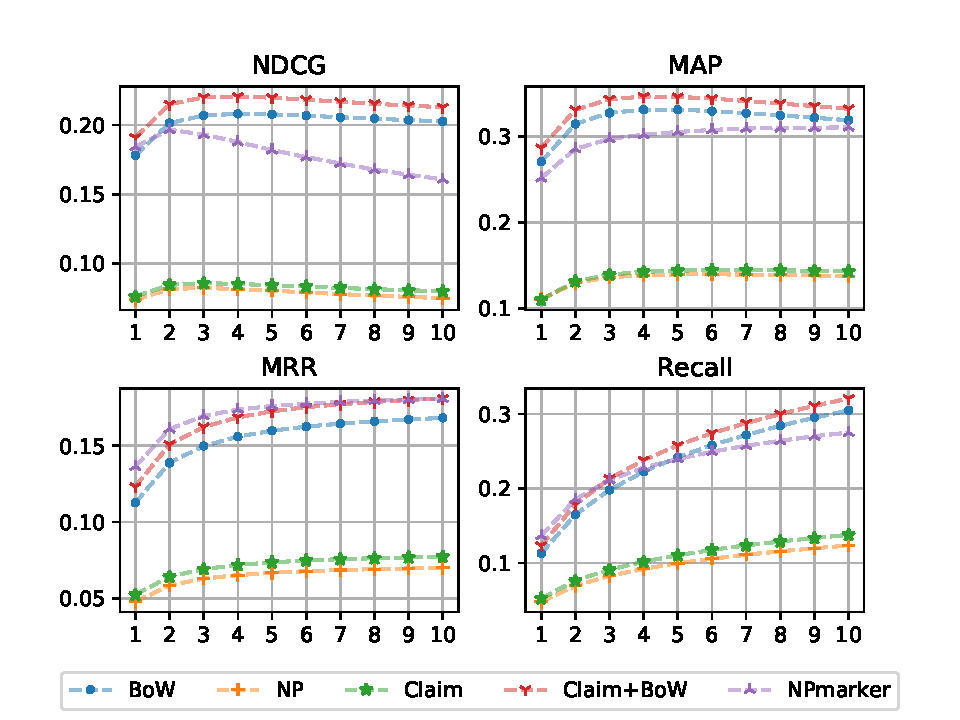
\includegraphics[width=.9\textwidth]{figures/evaluation/arXiv_CS_select.pdf}
  \label{fig:evalarxiv}
  \caption{Evaluation using arXiv.}
%\end{figure}

%\begin{figure}
  \centering
    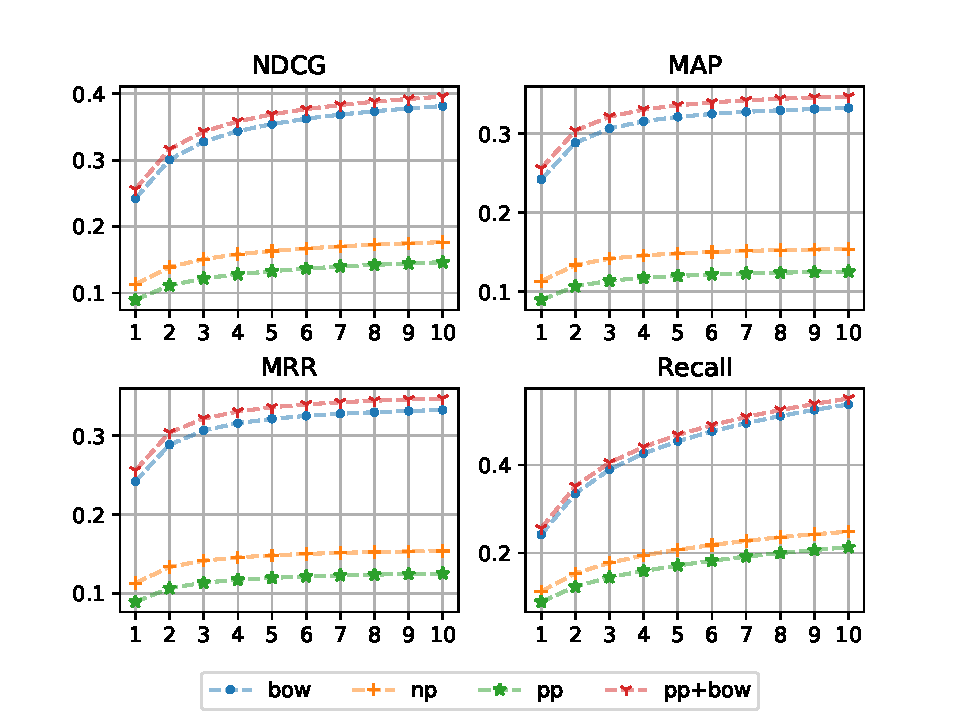
\includegraphics[width=.9\textwidth]{figures/evaluation/MAG_CS_es_wAbs_3M.pdf}
  \label{fig:evalmag}
  \caption{Evaluation using the MAG.}
\end{figure}

\begin{figure}
  \centering
    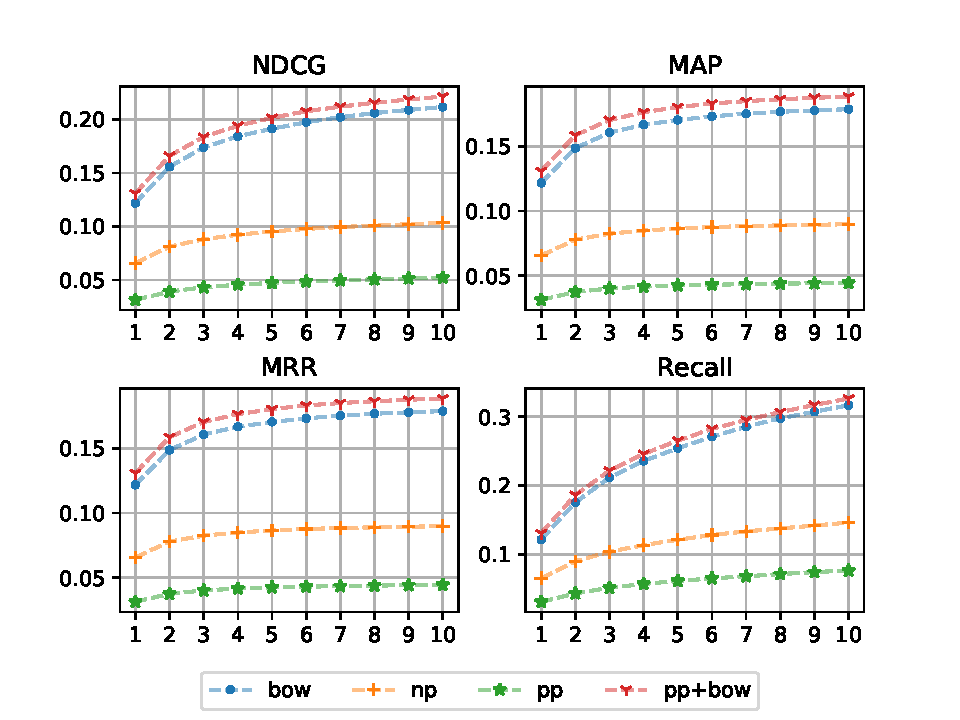
\includegraphics[width=.9\textwidth]{figures/evaluation/RefSeer.pdf}
  \label{fig:evalrefseer}
  \caption{Evaluation using RefSeer.}
%\end{figure}

%\begin{figure}
  \centering
    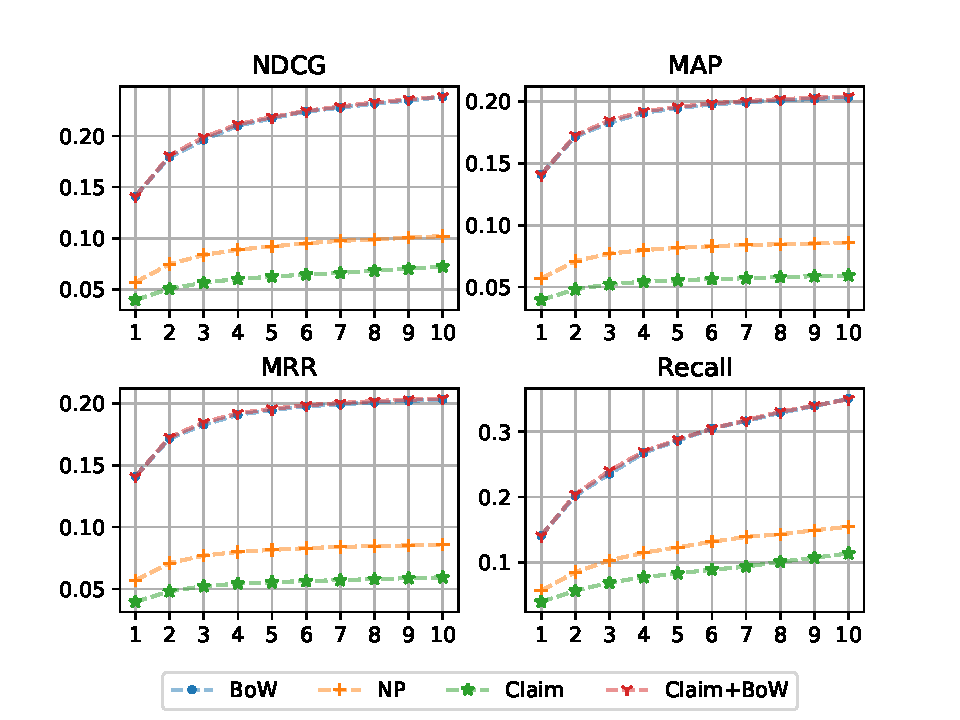
\includegraphics[width=.9\textwidth]{figures/evaluation/ACL.pdf}
  \label{fig:evalacl}
  \caption{Evaluation using ACL-ARC.}
\end{figure}

TFIDF baseline being hard to beat is consitent with observation in \cite{Beel2017}

\section{Online evaluation}\label{sec:oneval}
online online
